%!TEX root = ../rapport.tex
%!TEX encoding = UTF-8 Unicode

\chapter{Préparation}
\section*{Numéro 1}
\subsection*{a)}

Sachant que le signal MF possède une équation de la forme suivant :

\begin{equation}
	S_{MF} = A\cos(2\pi f_c t + 2\pi k_f \int m(t)dt)
\end{equation}

Et que le message envoyé est le suivant :
\begin{equation}
	m(t) = B \cos(2\pi f_m t)
\end{equation}

Alors l'intégrale du message est l'équation suivante :
\begin{equation}
	m(t)_i = \frac{B}{2\pi f_m}\sin(2\pi f_m t)
\end{equation}

Et le signal envoyé est le suivant :

\begin{equation}
	S_{MF} = A\cos(2\pi f_c t + \frac{B k_f}{f_m}\sin(2\pi f_m t))
\end{equation}


\begin{equation}
	S_{MF} = 10 \cos(2\pi 10^6 t + \frac{5 }{}\sin(2000\pi  t))
\end{equation}


\subsection*{b)}

L'indice de modulation peut être calculé a l'aide de l'équation suivante :

\begin{equation}
	\beta = \frac{\Delta}{f_m} = \frac{K_f max\{m(t)\}}{2\pi f_m}
\end{equation}

Comme le signal m(t) est un cosinus, son amplitude maximale est B

\begin{equation}
	\beta = \frac{5000}{2\pi 1000} = 0.7959
\end{equation}

\subsection*{c)}
La largeur de bande effective est donnée par l'équation suivante :

\begin{equation}
	LB \approx 2(f_m + \Delta f_c)= 2f_m(1+\beta)
\end{equation}

\begin{equation}
	LB \approx  2000(1+0.7959) = 3591.8
\end{equation}


\subsection*{d)}
Selon les tables de Bessel, pour un signal avec un $\beta$ de 0.7959, le signal va posséder un n de 3. Ainsi, la bande passante va être de $3f_m$, soit de 6 kHz.

\subsection*{e)}

Comme le spectre d'un signal FM est donné par l'équation suivante :

\begin{equation}
	e(t) = A \sum^\infty_{n=-\infty} J_n(\beta)\cos(2\pi(f_c+nf_m)t)
\end{equation}

et que pour un $\beta$ de 0.7959, nous avons les 4 valeurs suivantes de $J_n(\beta)$ : 0.85, 0.365, 0.074 et 0.0099. Alors nous aurons 7 raies spectrales comme le montre la figure \ref{schema1}.

\begin{figure}[htb]
\begin{center}
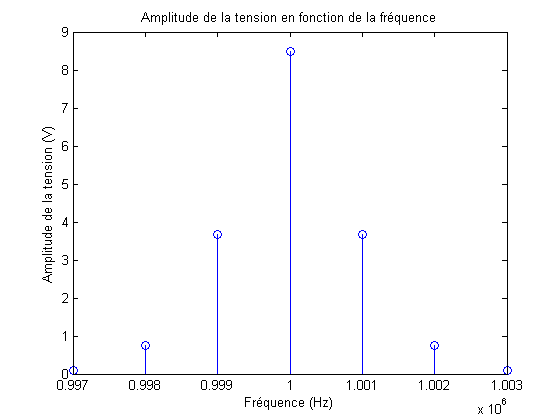
\includegraphics[scale=0.7]{no1e.png}
\caption{Figure représentant le spectre du signal FM demandé}
\label{schema1}
\end{center}
\end{figure}

